\subsection{Optimization using the Gradient}
One way of solving the optimization problem is through the use of the gradient. It indicates in which direction the steepest descent (or ascent) is found in an infinitesimal surrounding of a given starting point.

For a function \si{f(\vec{x})} with a change in \si{\vec{x}} of \si{\vec{\delta}}, the following can be obtained from the Taylor series.
%
\begin{flalign}
  f(\vec{x}+\vec{\delta}) &\approx f(\vec{x}) + \vec{g}^T \vec{\delta} + \frac{1}{2} \vec{\delta}^T \vec{H}\vec{\delta} &
\label{taylorApproximation}
\end{flalign}
%
\hspace{6mm} Where:\\
\begin{tabular}{ p{1cm} l l l}
& \si{\vec{g}} 					    	   & is the gradient \si{\nabla f(\vec{x})} & \\
& \si{\vec{H}} 					    	   & is the Hessian                         & \\
& \si{\vec{\delta}} 					   & is the change in \si{\vec{x}}          & \\
\end{tabular}

%Then the change in \si{f(x)} as \si{||\vec{\delta}||_2 \rightarrow 0} can be approximated as follows.
%%
%\begin{flalign}
%  \Delta f(x) &\approx \vec{g}^T \vec{\delta} = ||\vec{g}||_2 \ ||\vec{\delta}||_2 \ cos \theta &
%\label{changeInF}
%\end{flalign}
%%
%\hspace{6mm} Where:\\
%\begin{tabular}{ p{1cm} l l l}
%& \si{\theta} 					    	   & is the angle between \si{\vec{g}} and \si{\vec{\delta}}     & \\
%\end{tabular}

In gradient based methods, only the first order Taylor approximation is used, that is, the last term, \si{\frac{1}{2} \vec{\delta}^T \vec{H}\vec{\delta}} is discarded. If the derivative of the first order approximation is set to zero, the following is obtained.
%
\begin{flalign}
  \nabla\ f(\vec{x}+\vec{\delta}) &\approx \vec{g} = 0 &
\label{1stOrderTaylorApproximationParThetaEqZero}
\end{flalign}


That is, if the gradient of the function to be minimized is 0, a minimum or maximum exists as a candidate for a solution in this point. It follows that if standing in some point and computing the gradient in this point, then the gradient, \si{\vec{g}}, is the steepest ascent direction and the negative gradient, \si{-\vec{g}}, is the steepest descent direction. This only takes into account the immediate surroundings of the initially chosen point. A visualization of how the gradient points opposite to the minimum of an arbitrary function is seen on \figref{visualizationOfGradient}, which means that the negative gradient points to the minimum.


\begin{figure}[H] 
	\centering
	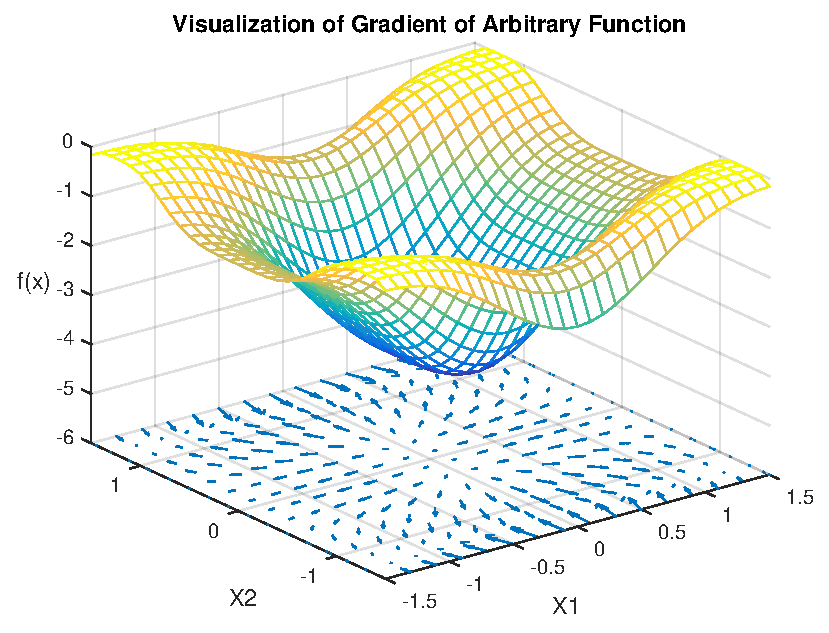
\includegraphics[width=.7\textwidth]{figures/visualizationOfGradient}
	\caption{Visualization of gradient of an arbitrary function.}
	\label{visualizationOfGradient}
\end{figure}

One way of implementation is to set a step-size which decides how far in the \si{-\vec{g}} direction to go. The step-size can then be scaled in each iteration to avoid taking too large steps as shown in \figref{SteepestDescendLargeStep} and \ref{SteepestDescendSmallStep}, where \si{x^*} is the value of \si{x} which minimizes \si{f(x)}, \si{x_0} is the starting point at which \si{-g} is computed and \si{x} is the point reached after the step.
%
\begin{minipage}{\linewidth}
	\begin{minipage}{0.45\linewidth}
		\begin{figure}[H]
			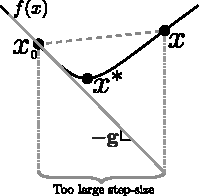
\includegraphics[scale=1.4]{figures/gradientDescendLargeStep2}
			\centering
			\captionsetup{justification=centering}
			\captionof{figure}{A too large step will cause the algorithm to step over the valley, resulting in a larger value of f(x) in the \si{-\vec{g}} direction.}
			\label{SteepestDescendLargeStep}
		\end{figure}
	\end{minipage}
	\hspace{0.03\linewidth}
	\begin{minipage}{0.45\linewidth}
		\begin{figure}[H]
			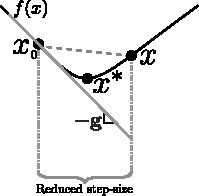
\includegraphics[scale=1.44]{figures/gradientDescendReducedStep2}
			\centering
			\captionsetup{justification=centering}
			\captionof{figure}{By going back and choosing a smaller step, a smaller value for f(x) is obtained.}
			\label{SteepestDescendSmallStep}
		\end{figure}
	\end{minipage}
\end{minipage}


The method does find a minimum. However, it converges to it rather slowly. An implementation where it is possible to directly retrieve the gradient of the function which is to be minimized, \si{f(\vec{x})}, is shown in \figref{steepestDescendEx}.

\begin{minipage}{\linewidth}
	\begin{minipage}{0.45\linewidth}
		\begin{figure}[H]
			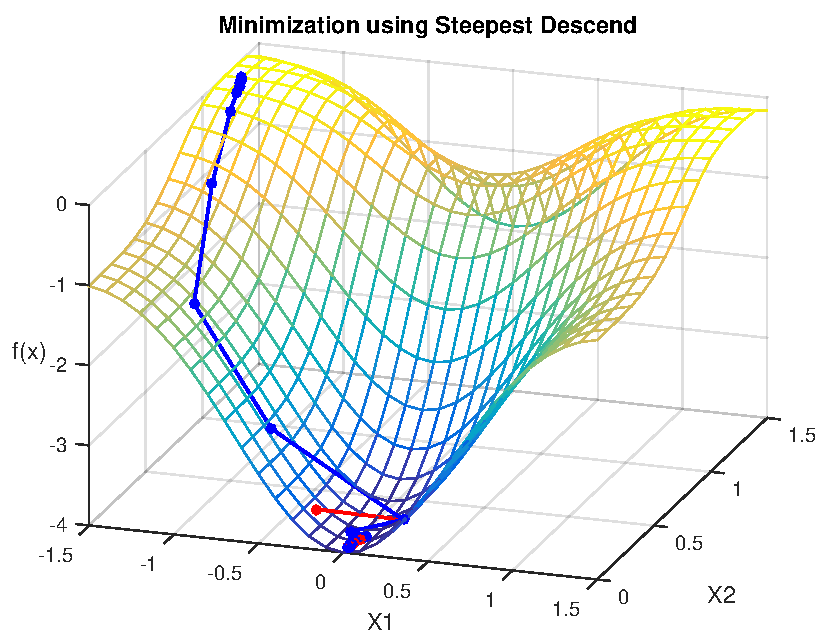
\includegraphics[scale=.6]{figures/steepestDescendEx}
			\centering
			\captionsetup{justification=centering}
			\captionof{figure}{An example of a direct implementation of a gradient optimization method. It steps over the valley and the step size is reduced in the red iteration.}
			\label{steepestDescendEx}
		\end{figure}
	\end{minipage}
	\hspace{0.03\linewidth}
	\begin{minipage}{0.45\linewidth}
		\begin{figure}[H]
			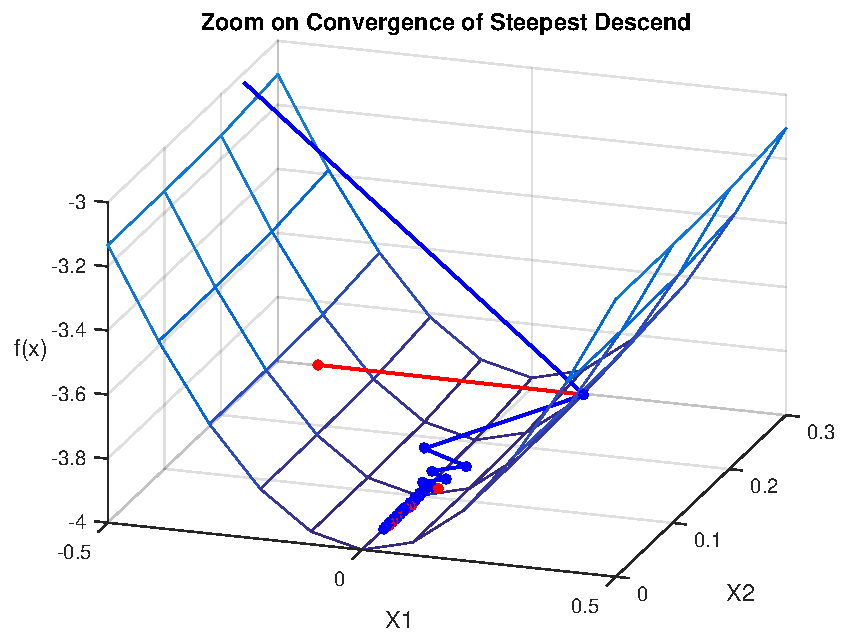
\includegraphics[scale=.6]{figures/steepestDesendExZoom}
			\centering
			\captionsetup{justification=centering}
			\captionof{figure}{From the zoom on the convergence, it is seen that many iterations (here 100) are needed using this method.\vspace{12pt}}
			\label{steepestDesendExZoom}
		\end{figure}
	\end{minipage}
\end{minipage}